\documentclass{article}

\usepackage{fancyhdr}
\usepackage{extramarks}
\usepackage{amsmath}
\usepackage{amsthm}
\usepackage{amsfonts}
\usepackage{tikz}
\usepackage[plain]{algorithm}
\usepackage{algpseudocode}
\usepackage{enumitem}
\usepackage{color}
\usepackage{tabularx}
\usepackage{graphicx}
\usepackage{adjustbox}
\usepackage{listings}
\usepackage{color}

\definecolor{dkgreen}{rgb}{0,0.6,0}
\definecolor{gray}{rgb}{0.5,0.5,0.5}
\definecolor{mauve}{rgb}{0.58,0,0.82}

\lstset{frame=tb,
  language=Java,
  aboveskip=3mm,
  belowskip=3mm,
  showstringspaces=false,
  columns=flexible,
  basicstyle={\small\ttfamily},
  numbers=none,
  numberstyle=\tiny\color{gray},
  keywordstyle=\color{blue},
  commentstyle=\color{dkgreen},
  stringstyle=\color{mauve},
  breaklines=true,
  breakatwhitespace=true,
  tabsize=3
}
\usetikzlibrary{automata,positioning}

%
% Basic Document Settings
%

\topmargin=-0.45in
\evensidemargin=0in
\oddsidemargin=0in
\textwidth=6.5in
\textheight=9.0in
\headsep=0.25in

\linespread{1.1}

\pagestyle{fancy}
\lhead{\hmwkAuthorName}
\chead{\hmwkClass\ - \hmwkTitle}
\cfoot{\thepage}

\renewcommand\headrulewidth{0.4pt}
\renewcommand\footrulewidth{0.4pt}

\setlength\parindent{0pt}

%
% Create Problem Sections
%

\newcommand{\enterProblemHeader}[1]{
    \nobreak\extramarks{}{Problem \arabic{#1} continued on next page\ldots}\nobreak{}
    \nobreak\extramarks{Problem \arabic{#1} (continued)}{Problem \arabic{#1} continued on next page\ldots}\nobreak{}
}

\newcommand{\exitProblemHeader}[1]{
    \nobreak\extramarks{Problem \arabic{#1} (continued)}{Problem \arabic{#1} continued on next page\ldots}\nobreak{}
    \stepcounter{#1}
    \nobreak\extramarks{Problem \arabic{#1}}{}\nobreak{}
}

\setcounter{secnumdepth}{0}
\newcounter{partCounter}
\newcounter{homeworkProblemCounter}
\setcounter{homeworkProblemCounter}{1}
\nobreak\extramarks{Problem \arabic{homeworkProblemCounter}}{}\nobreak{}

%
% Homework Problem Environment
%
% This environment takes an optional argument. When given, it will adjust the
% problem counter. This is useful for when the problems given for your
% assignment aren't sequential. See the last 3 problems of this template for an
% example.
%
\newenvironment{homeworkProblem}[1][-1]{
    \ifnum#1>0
        \setcounter{homeworkProblemCounter}{#1}
    \fi
    \section{Problem \arabic{homeworkProblemCounter}}
    \setcounter{partCounter}{1}
    \enterProblemHeader{homeworkProblemCounter}
}{
    \exitProblemHeader{homeworkProblemCounter}
}

%
% Homework Details
%   - Title
%   - Due date
%   - Class
%   - Section/Time
%   - Instructor
%   - Author
%

\newcommand{\hmwkTitle}{Homework\ \#5}
\newcommand{\hmwkDueDate}{}
\newcommand{\hmwkClass}{CS 351}
\newcommand{\hmwkClassTime}{Databases}
\newcommand{\hmwkClassInstructor}{Ben Mccamish}
\newcommand{\hmwkAuthorName}{\textbf{JT MUNDI}}
%
% Title Page
%

\title{
    \vspace{2in}
    \textmd{\textbf{\hmwkClass:\ \hmwkTitle}}\\
    \normalsize\vspace{0.1in}\large{\ \ \hmwkDueDate}\\
    \vspace{0.1in}\large{\textbf{\hmwkClassInstructor\ \hmwkClassTime}}\\
    \vspace{0.5in}
    \large{\textbf{\hmwkAuthorName}}\\
    \date{}
    \vfill
    
\includegraphics[width=0.4\textwidth]{logo.eps}
}



\renewcommand{\part}[1]{\textbf{\large Part \Alph{partCounter}}\stepcounter{partCounter}\\}

%
% Various Helper Commands
%

% Useful for algorithms
\newcommand{\alg}[1]{\textsc{\bfseries \footnotesize #1}}

% For derivatives
\newcommand{\deriv}[1]{\frac{\mathrm{d}}{\mathrm{d}x} (#1)}

% For partial derivatives
\newcommand{\pderiv}[2]{\frac{\partial}{\partial #1} (#2)}

% Integral dx
\newcommand{\dx}{\mathrm{d}x}

% Alias for the Solution section header
\newcommand{\solution}{\textbf{\large Solution}}

% Probability commands: Expectation, Variance, Covariance, Bias
\newcommand{\E}{\mathrm{E}}
\newcommand{\Var}{\mathrm{Var}}
\newcommand{\Cov}{\mathrm{Cov}}
\newcommand{\Bias}{\mathrm{Bias}}

\begin{document}

\maketitle

\pagebreak

\section{Schema}

The database schema was split up into four different relational tables to put the schema in Second Normal Form. First, the data for Genres, Keywords, Production Countries, Production Companies and Languages was put in an atomic form to ensure the database is in First Normal Form. Second, the four relational tables and four tables relating to those four relational tables were created to have no partial dependency on the primary keys. For each component of the primary key that acts as a determinant in a partial dependency, a new table with a copy of that component as the primary key was created. While these components were placed in the new tables, it was ensured that they remained in the original table as well. The determinants remain in the original table because they will be the foreign keys for the relationships that were needed to relate these new tables to the original table. All the relational tables have two foreign keys one from the movie table id of the movies and on id of each component such as genre, production, company and spoken language. The final database schema is in second normal form with no partial dependencies and completely atomic data.\newline 

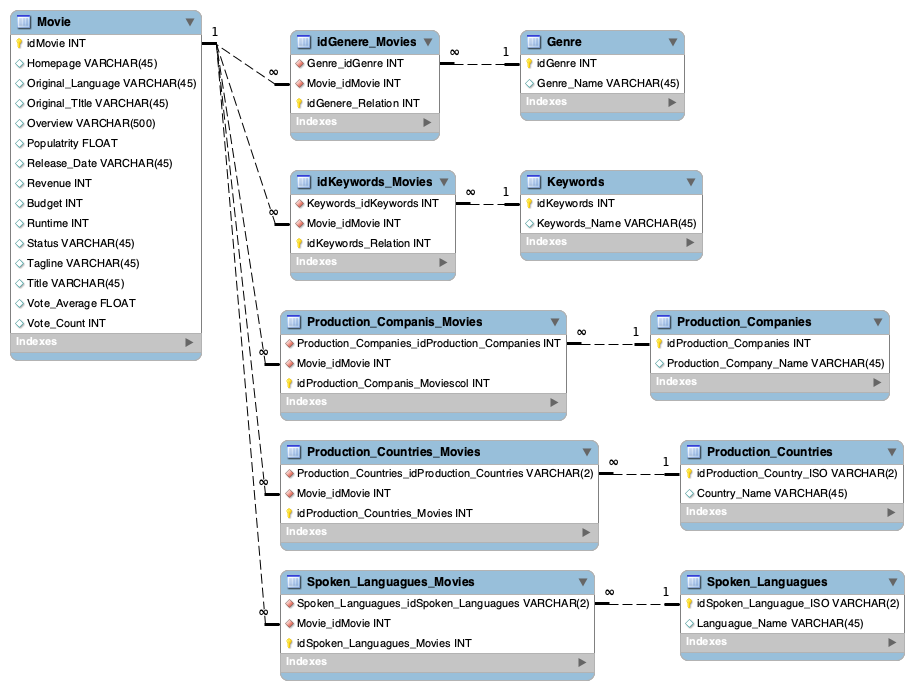
\includegraphics[width=1\textwidth]{ERR.png}

\textbf{Movie Table}

The movie table contains 15 attributes. idMovie is the primary key of the table. The table has one to many relationship with four relational tables.\newline 

\textbf{idGenre-Movies Table}

This table is a relational table between Movie table and Genres table. It creates a one to many relationship between Movie and Genre relationship table and many to one relationship between Genre relation table and Genre table. The idGenere-Movies table contains two foreign keys Genre-idGenere and Movie-idMovie and idGenere Relation is the primary key for this table. The primary key idGenere-Relation is iterated each time new keys are added to the table.\newline

\textbf{Genre Table}

The genre table contains two attributes idGenre and Genre-Name. idGenre is the primary key for this table related with one to many relationship with Genre-idGenre key in the idGenere-Movies table. Genre-Name contains the name of the genre associated with the idGenre.\newline

\textbf{idKeywords-Movies Table}

This table creates one to many relationship between Keywords and idMovie. The idKeywords-Movies table contains three attributes Keywords-idKeywords, Movie-idMovie and idKeywords-Relation. idKeywords-Relation is the primary key for this table.\newline

\textbf{Production-Companies-Movies Table}

This table is a relational table between Movie table and Production-Companies table. It creates a one to many relationship between Movie and Production-Companies relationship table and many to one relationship between Production-Companies-Movies relation table and Production-Companies table. The Production-Companies-Movies table contains two foreign keys Production-Companies-idProduction-Companies INT and Movie-idMovie and iProduction-Companis-Movies Relation is the primary key for this table. The primary keyProduction-Companis-Movies is iterated each time new keys are added to the table.\newline

\textbf{Production-Companies}

This table creates one to many relationship between Production companies and idMovie. The Production-Companies table contains three attributes Keywords-idKeywords, Movie-idMovie and idKeywords-Relation. idKeywords-Relation is the primary key for this table.\newline

\textbf{Production-Countries-Movies Table}

This table is a relational table between Movie table and Production-Countries table. The table has three attributes foreign key from Movie table Movie-idMovie and foreign key from Production-Countires idProduction-Country. The third attribute is the primary key for this table idProduction-Countires which is iterated on each insertion into the table. The both foreign keys form a relationship creating a many to many relation between Movie and Production-Countries table.\newline

\textbf{Production-Countries Table}
This table contains two attributes the primary key idProduction-Country and Country-Name which stores the name of the country where the movies was produced. The primary key has a one to many relationship with Production-Country-ID in the Production Countries relational table.\newline 

\textbf{Spoken-Languages-Movies Table}

This table is a relational table between Movie table and Spoken-Languages table. The table has three attributes foreign key from Movie table Movie-idMovie and foreign key from Spoken-Languages table idSpoken-Languages. The third attribute is the primary key for this table idSpoken-Languages-Movies which is iterated on each insertion into the table. The both foreign keys form a relationship creating a many to many relation between Movie and Spoken-Languages table.\newline 

\textbf{Spoken-Languages Table}
This table contains two attributes the primary key idPSpoken-Languages and Language-Name which stores the name of the language which was spoken in the movie. The primary key has a one to many relationship with Spoken-Language-idSpoken-Language in the Spoken-Languages-Movies relational table.\newline 

\pagebreak

\section{SQL Queries and Output}

\subsection{Query 1}
Average budget of all movies? Output includes just the average budget value.

\begin{lstlisting}[language=SQL]
SELECT 
  AVG(budget) 
FROM 
  movies.Movie
\end{lstlisting}

\textbf{Output}
\begin{lstlisting}
+---------------+
|  AVG(budget)  |
+---------------+
| 29045039.8753 |
+---------------+
\end{lstlisting}

\subsection{Query 2}
Show only the movies that were produced in the United States. Output includes the movie title and the production company name.

\begin{lstlisting}[language=SQL]
SELECT 
  DISTINCT(Original_TItle), 
  Production_Company_Name 
FROM 
  movies.Production_Countries_Movies AS CR 
  INNER JOIN movies.Movie as MM ON CR.Movie_idMovie = MM.idMovie 
  INNER JOIN movies.Production_Companis_Movies as PM ON PM.Movie_idMovie = MM.idMovie 
  INNER JOIN movies.Production_Companies as PC ON PC.idProduction_Companies = PM.Movie_idMovie 
WHERE 
  CR.Production_Countries_idProduction_Countries LIKE 'US' 
LIMIT 
  5;

\end{lstlisting}

\textbf{Output}
\begin{lstlisting}
+---------------------------------------------+------------------------------+
|                Original_TItle               |   Production_Company_Name    |
+---------------------------------------------+------------------------------+
|  Pirates of the Caribbean: At World''s End  |      Live Entertainment      |
|                 Spider-Man 3                |       TriStar Pictures       |
| Pirates of the Caribbean: Dead Man''s Chest |    Sony Pictures Classics    |
|   The Chronicles of Narnia: Prince Caspian  | Goldsmith-Thomas Productions |
| Pirates of the Caribbean: On Stranger Tides |   Zanuck/Brown Productions   |
+---------------------------------------------+------------------------------+
\end{lstlisting}

\subsection{Query 3}
Show the top 5 movies that made the most revenue. Output includes the movie title and how much revenue it brought in.

\begin{lstlisting}[language=SQL]
SELECT 
  Original_TItle, 
  Revenue 
FROM 
  movies.Movie as M 
ORDER BY 
  M.Revenue DESC 
LIMIT 
  5;
\end{lstlisting}

\textbf{Output}
\begin{lstlisting}
+----------------+------------+
| Original_TItle |  Revenue   |
+----------------+------------+
|     Avatar     | 2787965087 |
|    Titanic     | 1845034188 |
|  The Avengers  | 1519557910 |
| Jurassic World | 1513528810 |
|   Furious 7    | 1506249360 |
+----------------+------------+

\end{lstlisting}

Query 4 on next page.

\pagebreak

\subsection{Query 4}
What movies have both the genre Science Fiction and Mystery. Output includes the movie title and all genres associated with that movie.

\begin{lstlisting}[language=SQL]
SELECT 
  Title, 
  GROUP_CONCAT(Genre_Name SEPARATOR ', ') 
FROM 
  (
    SELECT 
      MY.Movie_idMovie 
    FROM 
      (
        SELECT 
          Movie_idMovie 
        FROM 
          movies.idGenere_Movies AS GSF 
        WHERE 
          GSF.Genre_idGenre = 9648
      ) AS SF 
      INNER JOIN movies.idGenere_Movies AS MY ON MY.Movie_idMovie = SF.Movie_idMovie 
    WHERE 
      MY.Genre_idGenre = 878
  ) AS F 
  INNER JOIN movies.Movie as M ON M.idMovie = F.Movie_idMovie 
  INNER JOIN movies.idGenere_Movies as G ON G.Movie_idMovie = M.idMovie 
  INNER JOIN movies.Genre as FG ON FG.idGenre = G.Genre_idGenre 
GROUP BY 
  Title 
LIMIT 
  5;
\end{lstlisting}

\textbf{Output}
\begin{lstlisting}
+--------------------------------------------+-------------------------------------------+
|                   Title                    |  GROUP_CONCAT(Genre_Name SEPARATOR ', ')  |
+--------------------------------------------+-------------------------------------------+
|           2001: A Space Odyssey            |    Science Fiction, Mystery, Adventure    |
|           Atlas Shrugged Part II           |      Drama, Science Fiction, Mystery      |
| Atlas Shrugged Part III: Who is John Galt? |      Science Fiction, Mystery, Drama      |
|       Beneath the Planet of the Apes       |    Adventure, Science Fiction, Mystery    |
|                 Blindness                  | Mystery, Science Fiction, Thriller, Drama |
+--------------------------------------------+-------------------------------------------+
\end{lstlisting}

\pagebreak

\subsection{Query 5}
Find the movies that have a popularity greater than the average popularity.Output includes the movie title and their popularity.
\begin{lstlisting}[language=SQL]
SELECT 
  Title, 
  Populatrity 
FROM 
  movies.Movie 
WHERE 
  Movie.Populatrity > (
    SELECT 
      AVG(Movie.Populatrity) 
    FROM 
      movies.Movie
  ) 
ORDER BY 
  Movie.Populatrity DESC 
LIMIT 
  5;

\end{lstlisting}

\textbf{Output}
\begin{lstlisting}
+-------------------------+-------------+
|          Title          | Populatrity |
+-------------------------+-------------+
|         Minions         |   875.581   |
|       Interstellar      |   724.248   |
|         Deadpool        |    514.57   |
| Guardians of the Galaxy |   481.099   |
|    Mad Max: Fury Road   |   434.279   |
+-------------------------+-------------+

\end{lstlisting}









\end{document}